I will begin this chapter with a less formal introduction to traditional rules and rule sets given in \ref{rulesandrulesets}.
Following it, I will go into more detail of belief rule-based systems giving a more formal presentation of the central ideas of belief-rule based
systems in \ref{belifrules}, \ref{inputtransformation}, and \ref{inference}. In \ref{inpractice}, I will show how a belief rule-based system can be built,
and in \ref{training} I will show how the system can be adaptively trained. I will conclude this chapter in \ref{numerical} with a numerical example, tying all the presented central ideas of belief rule-based systems
into  a practical application, and I will also present existing real life applications with belief rule-based systems.

{\color{red}
More motivation of why BRB systems are chosen here.}

The formal presentation of belief-rule based systems given in this chapter is based on the RIMER
method \cite{rimer2006}.

\section{Rules and rule sets}

{\color{red}I hope this sort of informal introduction giving an intuitive introduction to the main topic to be discussed
is appropriate in a thesis. I would skip this in a journal article.}

\label{rulesandrulesets}
Rules are a natural way of conveying information on how an agent or system should work according to its' surrounding environment.
A rule can be as simple as an if... then... statement; such a rule could be for example:

\begin{displayquote}
\textbf{Rule 1:} ``\textit{If it rains outside, bring an umbrella.}``.
\end{displayquote}

%However, such rules are strict. What if Bob is not sure if it is going to rain? Should he still take an umbrella if the sky looks dark?
%Belief-rule based systems are meant to tackle such scenarios. They extend the idea of rules to include a certain degree of belief to each rule.
%Then, given an observation, such as, how dark the sky looks, a belief-rule based system can give an answer that Bob should probably bring an umbrella,
%if he decides to venture outside.
A rule consists of three elements: the precedent, the condition, and the consequent. Take rule 1 as an example.
Suppose there was an agent named Bob who is contemplating whether he should bring an umbrella
outside or not. The precedent in the example should give a definite answer to the question implied by the condition of
the rule "if it rains". The question implied is "Does it rain?".
Therefore, Bob needs to look outside and see if it rains or not; he needs information from the surrounding environment.
Using the observed precedent and the condition, the rule can be resolved: If bob observes rain, he 
should bring an umbrella outside.

However, the rule in the previous example does not state anything
regarding the case when it does not rain outside. One could argue that the rule implicitly suggests to not bring an umbrella
in the absence of rain,
but it is not an explicit consequent of the rule in the case of no rain. To cover the case of no rain,
an additional rule should be stated:

\begin{displayquote}
\textbf{Rule 2:} ``\textit{If it does not rain outside, do not bring an umbrella.}``.
\end{displayquote}

In turn, rule 2 does not state anything regarding the case when it does rain outside. 
For Bob to have a coherent set of actions to take, whether to bring an umbrella outside or not,
the rules 1 and 2 should be combined into a single rule set:

\begin{displayquote}
\textbf{Rule set 1:}
$
\begin{cases}
``\textit{If it rains outside, bring an umbrella.}`` \\
``\textit{If it does not rain outside, do not bring an umbrella.}`` 
\end{cases}
$
\end{displayquote}

Rule set 1 is now a complete rule set; a definite consequent follows all possible precedents, namely "It rains outside."
and "It does not rain outside.". If there was a third precedent in the example, for example: "It might be raining outside", rule set 1
would be incomplete and is said to contain a degree of ignorance: It does not state what to do in the case when the observation of rain
is indefinite.

That being said, in real life, observations are seldom definitive. To cover all possible cases of
different observations, made by Bob in rule set 1,
would mean an addition of an indefinite number of rules, with the precedents covering all possible cases.
In practice, trying to cover all cases is an exercise in futility.

Could the conditions of rules in a rule set have a degree of truthiness associated to them, instead of being simply true of false?
Could such rule set cover a continuous range of observations and outcomes?
Is it possible to infer an appropriate consequent from such a rule set, and how to interpret the outcome?
This is where belief rule-based systems come into play.

\section{Belief rules}
\label{belifrules}
In a belief rule $R$, the precedent is defined as a set of finite arrays of referential values, and the consequent
is defined as a single finite array of referential values. In this thesis, it is assumed that these referential values
are real numbers.

Following the RIMER approach \cite{rimer2006} to define a belief rule,
a referential array set $A$, called a packet precedent, with finite arrays $A_i$, is defined as the precedent of a 
belief rule:

\begin{equation}
\label{eq:A_set_def}
    A = \Set{ A_i = \Set{A_{i, n} \mid \forall n \in \left[1, \left|A_i\right| \right]}
    \mid \forall i \in \left[1, T \right] }, \quad\text{where}\quad i, n, T \in \mathbb{N}.
\end{equation}

And an array of finite values, $D$, is defined as the consequent in a belief rule:

\begin{equation}
\label{eq:D_set_def}
    D = \Set{D_j \mid \forall j \in \left[1, N \right] }, \quad\text{where}\quad j, N \in \mathbb{N}.
\end{equation}

In \eqref{eq:A_set_def} and \eqref{eq:D_set_def}, $T$ is the total number of attributes in an observation, $A_i$ is the array of possible  referential values
for the $i$th attribute in an input, $\left|A_i\right|$ is the number of referential values for the $i$th attribute in an input,
and $N$ represent the total number of referential values for the consequent.

The input to a belief rule is defined as $X$, which is an array of precedent values
for $T$ attributes defined as

\begin{equation}
    \label{eq:X_input}
    X = \Set{ x_i \mid \forall i \in \left[1, T \right]}, \quad\text{where}\quad i \in \mathbb{N}.
\end{equation}

Attributes $x_i$ in \eqref{eq:X_input} take values equal to the values defined in
the finite arrays $A_i$ present in the packet precedent $A$ in \eqref{eq:A_set_def}.

The condition of a belief rule can be defined as a logical relationship $F$ between the input $X$, and
the packet precedent $A$ as

\begin{equation}
    \label{eq:logical}
    F : x_1\;\text{is}\;A_1^*\;\land\;x_2\;\text{is}\;A_2^*\;\land\dots\land\;x_T\;\text{is}\;A_T^*,
\end{equation}

where $A_i^* \in A_i$ represents the referential value taken by the attribute $x_i$ in the belief rule.

The logical relation $\land$ present in \eqref{eq:logical}, could be replaced by some other logical relation, but in this thesis,
the RIMER approach is followed, which uses the $\land$ relation.

Finally, a single belief rule can be defined as

\begin{align}
\begin{split}
    \label{eq:singlerule}
    & \text{IF}\; x_1\; \text{is}\; A_1^k\; \land\; x_2\; \text{is}\; A_2^k\; \land\; \dots\; \land\; x_{T_k}\; \text{is}\; A_{T_k}^k, \\
    R_k:\quad & \text{THEN}\; \Set{\left( D_i, \beta_{i, k} \right) \mid \forall i \in \left[1, N \right]}, \\
    & \text{with an associated rule weight}\; \theta_k, \\
    & \text{and attribute weights}\; \Set{\delta_{i, k} \mid \forall i \in \left[ 1, T_k \right]},
\end{split}
\end{align}

with the property

\begin{equation}
    \label{eq:betasum}
    \sum_{i=1}^{N} \beta_{i, k} \leq 1.
\end{equation}

% The single rule \eqref{singlerule} can be then be generalized to a finite set of $L \in \mathbb{N}$ belief rules as

In \eqref{eq:singlerule}, it is understood that the rule $R_k$ has its' own packet precedent $A^k \subset A$, with
$T_k$ referential value vectors, defined. $A_i^k$, for which $A_i^k \in A_i \in A^k$, is then the value taken by the $i$th attribute in the input to the $k$th rule.
Rule weight $\theta_k$ represents how important the rule $R_k$ is, usually compared to other rules.
The attribute weights
$\delta_{i,k}$ represent how important attributes are compared to each other in the rule $R_k$. The rule weights and attribute weights will
be discussed later.

The belief degrees $\beta_{i, k}$ represent the degree of belief for the consequent
$D_i$ to be true in rule $R_k$. The output of a belief rule is therefore a belief distribution.
Property \eqref{eq:betasum} is equal to one when the output of a rule can be fully expressed using
the consequents referential values $D_i$. Otherwise, a degree of ignorance is present in the consequent of the rule.

Using the rule defined in \eqref{eq:singlerule}, a belief rule base, consisting of $L$ belief rules, can be established
and is represented as

\begin{equation}
    \label{eq:genericrule}
    R = \braket{X, A, D, F}.
\end{equation}

Inference can then be performed on belief rule base $R$ for a specific input vector $X$.
The inference mechanism, and the generation on the input vector,
are discussed in the following sections.

%For a real valued observation $X$ to be usable with a belief rule, the observation must be first expressed as a belief distribution over
%the set of referential values defined for the precedents in the rule. It is therefore assumed that $A$ is defined in a way, which allows the expression
%of the observation $X$. As presented in \ref{TODO}, the observation $X$ can be transformed to the following distribution

%\begin{equation}
%    \alpha = \Set{
%    \min{\left(
%    \max{\left( \frac{A_{i+1} - X}{A_{i+1} - A_{i}}, 0 \right)},\:
%    \max{\left( \frac{X - A_{i-1}}{A_i - A_{i-1}}, 0 \right)}
%    \right)}
%    \mid \forall i \in \left[1, T\right] },
%\end{equation}

%where $A_0 = A_T$ and $A_{T+1} = A_1$.

\section{Input transformation}
\label{inputtransformation}
{\color{red}
Belief distributions and belief degrees are presented, and the link to belief rules is established.
}

Because the attribute values $x_i$ present in the input $X$ \eqref{eq:X_input} being restricted to the referential values present in $A_i$
for each attribute in a belief rule set, observed data in an observation

\begin{equation}
    \label{eq:observation}
    H = \Set{h_i \mid \forall i \in \left[1, T\right]}
\end{equation}

may, or may not be, usable directly in rules in a belief rule set. Expanding the vectors of referential values $A_i$ in
\eqref{eq:A_set_def} to include all possible values for each $h_i$ in
a rule set
is counterproductive, and borderline impossible with the assumption of the referential values for the precedents being real valued.
Therefore, observations are to be transformed into belief distributions, which convey a degree of belief for each observed attribute to
be assessed to a certain referential value in the precedent of a belief rule. In this thesis, it is assumed that all observed 
inputs are real valued, in other words $\forall h_i \in H, h_i \in \mathbb{R}$, and the handling of qualitative observations is not necessary.

However, it is worth mentioning that qualitative observations can be used as input to belief rules. A belief structure must be
defined, which works as a mapping between the qualitative observations and the inputs to a belief rule.

For a single observed attribute
$h_i$, and the precedent referential values $A_i$, the observed attribute is transformed into a belief distribution

\begin{equation}
\label{eq:single_beliefdist}
s_i = \Set{\left(A_{i, n}, \alpha_{i, n}\right) \mid \forall n \in \left[1, \left|A_i\right|\right]},
\end{equation}

where $\alpha_{i,n}$ represents the belief degree that the attribute $h_i$ is assessed to the referential value
$A_{i,n}$. The belief degrees $\alpha_{i, n}$ can be calculated as follows \cite{Chen2011}:

\begin{equation}
    \label{eq:single_transform}
    \alpha_{i, n} = \Set{
    \min{\left(
    \max{\left( \frac{A_{i, n+1} - h_i}{A_{i, n+1} - A_{i, n}}, 0 \right)},\:
    \max{\left( \frac{h_i - A_{i, n-1}}{A_{i, n} - A_{i, n-1}}, 0 \right)}
    \right)}
    \mid \forall n \in \left[1, \left|A_i\right|\right] },
\end{equation}

where $A_{i, 0} = A_T$ and $A_{i, \left|A_i\right|} = A_1$. The belief degrees calculated using
\eqref{eq:single_transform} have the property

\begin{equation}
    \label{eq:alpha_sum}
    \sum_{n=1}^{\left|A_i\right|} \alpha_{i, n} \leq 1.
\end{equation}

The sum in property \eqref{eq:alpha_sum} is equal to one, when an observed attribute $h_i$ can be fully assessed to
the values defined in the precedent referential values $A_i$. If the sum is less than one,
some degree of ignorance is present; the attribute $h_i$ cannot be fully assessed to the referential
values in $A_i$.

For multiple inputs, the belief distribution in \eqref{eq:single_beliefdist} can be generalized to a set
of belief distributions

\begin{equation}
\label{eq:multi_beliefdist}
    S = \Set{
    \Set{
    \left(A_{i, n}, \alpha_{i, n}\right) \mid \forall n \in \left[1, \left|A_i\right|\right]
    } \mid \forall i \in \left[ 1, T \right]
    }.
\end{equation}

\section{Inference mechanism}
\label{inference}
{\color{red}
How to use evidential reasoning to reason about a BRB system. Formulas are shown, not derived, on how to transform an input to a BRB system,
how to calculate activation weights of
a BRB system using the transformed input, and how the belief degrees can then be calculated using the activation weights. What is a belief rule expression matrix?
}

So far, the concept of a belief rule, and how to transform an observation into an input to a belief rule, has been defined.
To really make use of a belief rule base, an inference mechanism is needed.

For a belief rule base of $L$ total rules, the values of the rule weights $\theta_k$, belief degrees $\beta_{i, k}$, and attribute
wights $\delta_{i,k}$ are assumed to be known\footnote{Either given by an expert or learned.}. An activation weight $w_k$ can then be calculated for each rule
as follows \cite{Chen2011}:

\begin{equation}
\label{eq:activationweight}
    w_k =
    \frac
    {\theta_k\prod_{i=1}^{T_k}\left(\alpha_{i, n}^k\right)^{\bar{\delta}_{i, k}}}
    {\sum_{l=1}^{L}\left[\theta_l\prod_{i=1}^{T_l}\left(\alpha_{i, n}^l\right)^{\bar{\delta}_{i, l}}\right]},
\end{equation}

where

\begin{equation}
    \label{eq:normdelta}
    \bar{\delta}_{i, m} = \frac{\delta_{i, m}}{\max_{\forall i \in T_m}\left(\delta_{i, m}\right)}.
\end{equation}

In \eqref{eq:activationweight} the term $\alpha_{i, n}^k$ indicates how the $i$th attribute, in an input to the $k$th
rule in a belief rule base, matches the precedent value $A_i^k$ defined in the rule. 
The product present in the nominator of \eqref{eq:activationweight} is an aggregation of the belief degrees 
defined in \eqref{eq:multi_beliefdist}
for each attribute present in the input of the rule. Since the logical relation of the precedents, in a belief rule, 
is assumed to be the `AND` connective, $\land$, the belief degrees are combined using a product. In other words,
a belief rule $k$ is active, meaning it has a non-zero activation weight, only when all of the attributes present in the input to the rule can be associated
to the precedent
referential values $A_1^k, A_2^k, \dots, A_{T_k}^k$ present in the condition of the rule. Otherwise, the rule activation
weight $w_k$ will be zero, and the rule is not active for the given input.

Moreover, the importance of each attribute in the $k$th belief rule, is indicated by the attribute weights 
$\delta_{i, k}$, which are normalized 
to $\bar{\delta}_{i, k}$ according to \eqref{eq:normdelta}. Thus, in the $k$th rule, an attribute with a normalized attribute
weight of $1$ is deemed the most
important, affecting the activation weight in \eqref{eq:activationweight} substantially, while
an attribute with an activation weight of $0$ has no impact on the activation weight. This is a direct consequent of the nature of the
exponential function present in the multiplicands in \eqref{eq:activationweight}.

Lastly, the rule weight $\theta_k$ in \eqref{eq:activationweight} represents the importance of the $k$th rule
in the rule base. The value can be arbitrary, but in this thesis, it is assumed that the weights are positive, and normalized such that
they sum to unity:

\begin{equation}
    \label{eq:thetasum}
    \sum_{k=1}^L \theta_k = 1.
\end{equation}

The normalization for the rule weights in \eqref{eq:thetasum} is done mostly out of convenience.

After calculating the rule weights, evidential reasoning can be used, as in inference mechanism,
to combine activated rules, and infer an output vector of a belief rule base for a certain input
vector. The inference mechanism presented in based on the Dempster-Shafer theory, fuzzy set theory, and
decision theory, as presented in \cite{Chen2011}. This thesis will not dive further into the details
of the inference mechanism, and will simply present relevant results.

To aggregate the outputs of the different belief rules in a rule base, a combined belief degree
$\beta_n$ is calculated to produce a final belief distribution

\begin{equation}
    \label{eq:outputdist}
    S(y) = \Set{\left(D_n, \beta_n \right) \mid \forall n \in \left[1, N \right]}
\end{equation}

on the referential values $D$, representing an output $y$. In this thesis, it is assumed that $y$
is always numerical. To get $y$ from the belief distribution in \eqref{eq:outputdist}, a utility
function

\begin{equation}
    \label{eq:outpututility}
    u: D_n \to \mathbb{R}
\end{equation}

must be defined. After the utility $u$ is defined, the numerical output associated to the
belief distribution \eqref{eq:outputdist} system can be
calculates to be

\begin{equation}
    \label{eq:utilitysum}
    y = \sum_{n=1}^{N}u(D_n)\beta_n.
\end{equation}

According to
\cite{Chen2011}, and assuming that the rules in a rule base are independent of each other,
the combined belief degrees can be calculated as follows:

\begin{equation}
    \label{eq:combinedbelief}
    \beta_n =
    \frac
    {\prod_{k=1}^L(w_k\beta_{n,k}+1-w_k\sum_{i=1}^N\beta_{i,k}) -
    \prod_{k=1}^L(1 - w_k\sum_{i=1}^N\beta_{i,k})}
    {\sum_{j=1}^N\prod_{k=1}^L(w_k\beta_{j,k}+1-w_k\sum_{i=1}^N\beta_{i,k}) -
    (N-1)\prod_{k=1}^L(1-w_k\sum_{i=1}^N\beta_{i,k})-\prod_{k=1}^L(1-w_k)}.
\end{equation}

It is evident in \eqref{eq:combinedbelief} that when a rule $k$ is not activate with an activation weight $w_k = 0$,
the combined belief $\beta_n$ will not be affected by rule $k$. Furthermore, in \eqref{eq:combinedbelief}, if a rule $k$
is active, and the rule has an individual belief degree $\beta_{n,k}$ associated to the output $D_n$ in the rule, then the overall output must be
assessed to $D_n$, at least to some degree. The magnitude of the degree of a rule $k$ affecting the combined belief degree, is
affected both by the importance of the $k$th rule to the overall output, and the degree of activation of the precedent in the $k$th
rule by an input vector.

\section{Belief rule-based systems in practice}
\label{inpractice}
In the previous chapters various concepts, like a belief rule base, input transformation, and inference mechanism, have been introduced.
A belief-rule based (BRB) system is a system that combines those concepts. In figure \ref{fig:brbschematic},
a schematic representation of a BRB system is given illustrating its' various components, and how the components depend on
each other through different variables. In essence, BRB systems model relationships between precedent and consequent attributes, given an
input based on an observation.

\begin{figure}[htp]
    \centering
    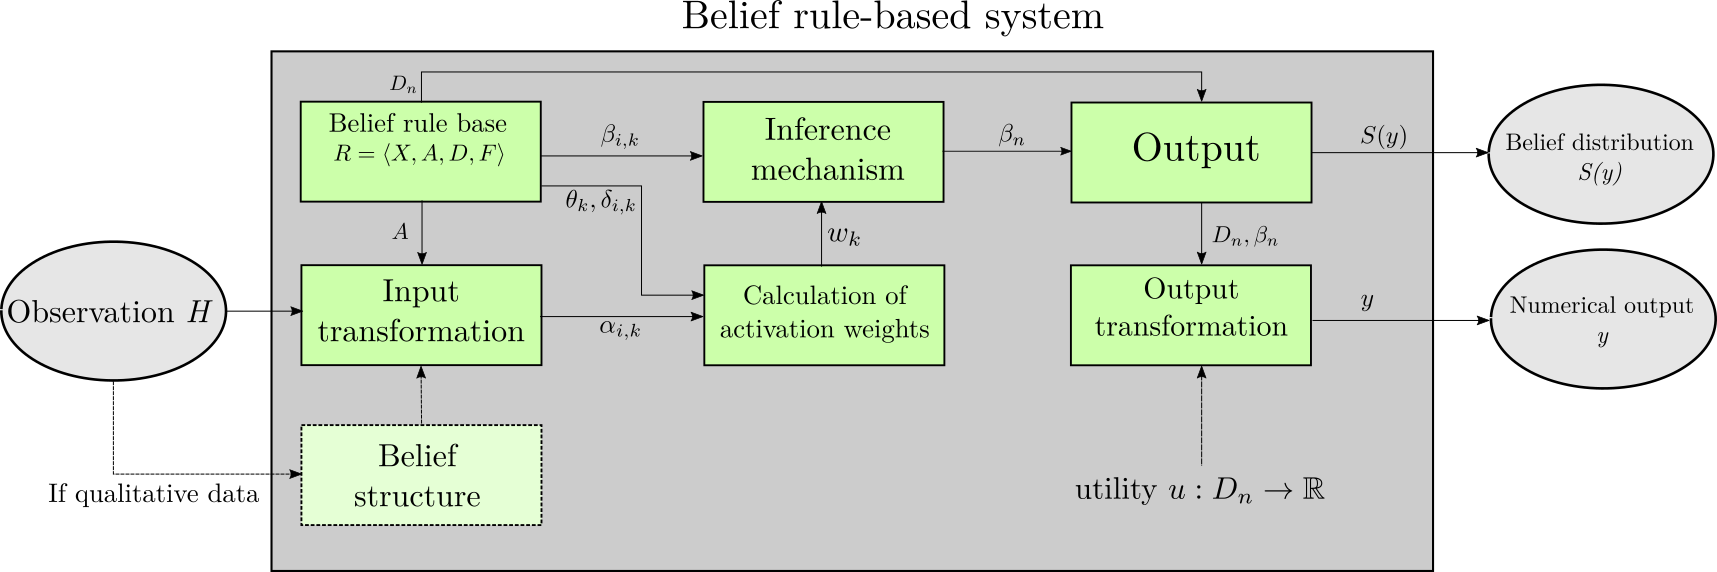
\includegraphics[width=15cm]{contents/brb_structure.png}
    \caption{\emph{A schematic representation of the components of a BRB system. The arrows represent the
    dependencies between the components.}}
    \label{fig:brbschematic}
\end{figure}

To build a BRB system, an initial\footnote{Before any training is done.} rule base must be build.
As an example, suppose a BRB system, which models the relationship of a numerical input $X$ of two attributes, $x_1$ and $x_2$ to some numerical 
output $y$, which
in turn will be represented by three consequent referential values $D = \Set{D_1, D_2, D_3}$.
The packet precedent $A$ of
such a system has two components, namely $A_1$ and $A_2$. Furthermore, suppose that the components $A_1$ and $A_2$ contain both three
referential values, that is $A_1 = \Set{A_{1,1}, A_{1,2}, A_{1,3}}$ and $A_2 = \Set{A_{2,1}, A_{2,2}, A_{2,3}}$. From these precedents, a total
of nine belief rules can be constructed. The nine rules cover all the cases of possible value pairs of the input $X = (x_1, x_2)$, where
the attributes $x_1$ and $x_2$ take values available in the vectors $A_1$ and $A_2$ respectively. An example of such a belief rule
according to \eqref{eq:singlerule} is

\begin{align}
\begin{split}
    \label{eq:examplerule}
    & \text{IF}\; x_1\; \text{is}\; A_1^1\; \land\; x_2\; \text{is}\; A_2^1\;, \\
    R_1:\quad & \text{THEN}\; \Set{\left( D_i, \beta_{i, 1} \right) \mid \forall i \in \left[1, 3 \right]}, \\
    & \text{with an associated rule weight}\; \theta_1, \\
    & \text{and attribute weights}\; \Set{\delta_{i, 1} \mid \forall i \in \left[ 1, 2 \right]}.
\end{split}
\end{align}

The possible combinations of the precedent referential values present in the conditional of the rule can be calculated using the Cartesian product
over the two referential value vectors $A_1$ and $A_2$

\begin{equation}
    \label{eq:cartesianexample}
    A_1 \otimes A_2 = \Set{(a_1, a_2) \mid a_1 \in A_1\;\text{and}\;a_2 \in A_2},
\end{equation}

which results in nine different combinations.

\eqref{eq:cartesianexample} can be generalized for any packet precedent, with an any
number of referential value vectors $T$ as

\begin{equation}
    \label{eq:cartesiangeneral}
    \bigotimes_{i=1}^{T} A_i = \Set{(a_1, a_2, \dots, a_T) \mid a_1 \in A_1\;\text{and}\;a_2 \in A_2\dots\;\text{and}\;a_T \in A_T}.
\end{equation}

The total number of rules $L$, in a rule base with the packet precedent $A$, is then the total number of the combinations present in the Cartesian product 
\eqref{eq:cartesiangeneral}, or equivalently

\begin{equation}
    \label{eq:totalrules}
    L = \prod_{i=1}^T\left|A_i\right|.
\end{equation}

Using \eqref{eq:totalrules} with the defined vectors $A_1$ and $A_2$, the total number of rules amounts to $L=9$ like previously stated.

Continuing the example, the belief degrees $\beta_{i,k}$, rule weights $\theta_k$, and attribute weights $\delta_{i,k}$ are yet to be defined.
The belief degrees $\beta_{i,k}$ can be assigned by an expert, or be inferred from existing data. For example, suppose the BRB system in this example
is trying to model the function

\begin{equation}
    \label{eq:examplefun}
    f: \mathbb{R}^2 \to \mathbb{R}; f(x_1, x_2) = x_1 + x_2. 
\end{equation}

Using $f$ defined in \eqref{eq:examplefun}, the numerical consequent for each possible combination of the precedents in \eqref{eq:cartesianexample} can
be calculated. However, the calculated value must be transformed into a belief distribution to produce the belief degrees $\beta_{i,k}$ for each
rule. It turns out that equation \eqref{eq:single_transform} can be used, with the calculated values using \eqref{eq:examplefun} for each rule,
to produce a belief distribution of $\beta_{i, k}$ over
the consequent values $D$ using the substitutions

\begin{equation}
     \alpha_{i,n} \to \beta_{i, k}, \;\text{and}\; A_{i,} \to D.
\end{equation}

This way all the belief degrees $\beta_{i,k}$, in each rule, can be calculated for the initial rule base.

The remaining rule weights $\theta_k$ and attribute weights $\delta_{i,k}$ cannot be calculated with \eqref{eq:examplefun}, and must be inferred in some
other way. In the light of this thesis, the rule weights and attribute weights, are always assumed to be

\begin{equation}
    \label{eq:assumedweights}
    \theta_k = \frac{1}{L}\;\text{and}\;\delta_{i,k} = 1,
\end{equation}

in the initial rule base. Assumption \eqref{eq:assumedweights} will be assumed for this example as well.

All the necessary components of the initial rule base have now been defined. Input transformation, for some observation
$H$, can be done using \eqref{eq:single_transform} and the defined packet precedent $A$, producing the belief degrees $\alpha_{i,k}$, which can
be used in conjunction with the rule weights $\theta_k$ and attribute weights $\delta_{i,k}$ to calculate the rule
activation weights $w_k$ using \eqref{eq:activationweight}. Information of the example's rule base can be summarized in a belief rule expression
matrix as shown in table \ref{tab:examplematrix}.

\begin{table}[h]
\centering
    \begin{tabular}{lccc}
    \toprule
    Input & \multicolumn{3}{l}{Belief output} \\
    \cline{2-4}
    & $D_1$ & $D_2$ & $D_3$ \\
    \midrule
    $A_1(w_1)$ & $\beta_{1,1}$ & $\beta_{2,1}$ & $\beta_{3,1}$ \\
    $A_2(w_2)$ & $\beta_{1,2}$ & $\beta_{2,2}$ & $\beta_{3,2}$ \\
    $A_3(w_3)$ & $\beta_{1,3}$ & $\beta_{2,3}$ & $\beta_{3,3}$ \\
    $A_4(w_4)$ & $\beta_{1,4}$ & $\beta_{2,4}$ & $\beta_{3,4}$ \\
    $A_5(w_5)$ & $\beta_{1,5}$ & $\beta_{2,5}$ & $\beta_{3,5}$ \\
    $A_6(w_6)$ & $\beta_{1,6}$ & $\beta_{2,6}$ & $\beta_{3,6}$ \\
    $A_7(w_7)$ & $\beta_{1,7}$ & $\beta_{2,7}$ & $\beta_{3,7}$ \\
    $A_8(w_8)$ & $\beta_{1,8}$ & $\beta_{2,8}$ & $\beta_{3,8}$ \\
    $A_9(w_9)$ & $\beta_{1,9}$ & $\beta_{2,9}$ & $\beta_{3,9}$ \\
    \bottomrule
    \end{tabular}
    \caption{\emph{A belief rule expression matrix summarizing the information of the rule base for a rule base with nine belief rules, and
    three consequent referential values.}}
    \label{tab:examplematrix}
\end{table}

Each row in the table \ref{tab:examplematrix} represents one 
rule in the rule base with the associated consequent belief degrees.
The first column in table \ref{tab:examplematrix} represents the inputs, which in the case of the example in this chapter means one of the pairs
of referential values emerging from the Cartesian product in \eqref{eq:cartesianexample}, to each rule with that rule's activation weight.

The information in table \ref{tab:examplematrix} for some input $X$, can now be used to infer the combined belief degrees of the BRB system using
\eqref{eq:combinedbelief} to produce the output of the system $S(y)$, as defined in \eqref{eq:outputdist}. Assuming a simple utility function, congruent
with \eqref{eq:outpututility},

\begin{equation}
    u(D_n) = D_n
\end{equation}

the numerical output of the BRB system can be finally calculated using \eqref{eq:utilitysum} and the calculated combined belief degrees $\beta_n$.


\section{Training belief rule-based systems}
\label{training}
{\color{red}
How input output pairs can be used to fine tune the parameters of a BRB system.
}

\section{Numerical example and existing applications}
\label{numerical}
{\color{red}
Finally, a simple numerical example is given, with a link to the source code to reproduce the results. I plan to model a non-linear function, and show,
the capability of a BRB system in modelling a non-linear system as a motivation. It is mentioned that the author has developed a simple software library to implement
trainable BRB models.
}